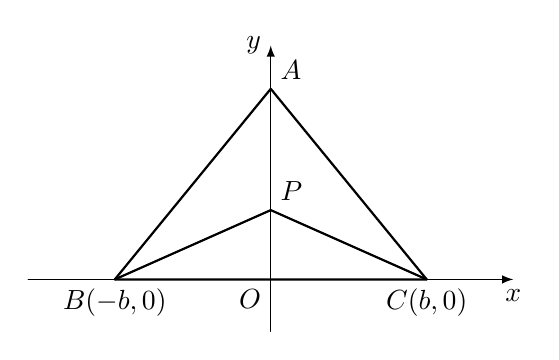
\begin{tikzpicture}[>=latex, scale=1.1, line join=round, line cap=round]
  % Axes
  \draw[->] (-2.8, 0) -- (2.8, 0) node[below] {$x$};
  \draw[->] (0, -0.6) -- (0, 2.7) node[left] {$y$};
  \node[below left] at (0, 0) {$O$};

  % Coordinates
  \coordinate (B) at (-1.8, 0);
  \coordinate (C) at (1.8, 0);
  \coordinate (A) at (0, 2.2);
  \coordinate (P) at (0, 0.8);

  % Triangle and segments
  \draw[thick] (B) -- (A) -- (C) -- cycle;
  \draw[thick] (B) -- (P) -- (C);

  % Labels
  \node[below] at (B) {$B(-b,0)$};
  \node[below] at (C) {$C(b,0)$};
  \node[above right] at (A) {$A$};
  \node[above right] at (P) {$P$};
\end{tikzpicture}
